\documentclass[]{article}
\usepackage[T1]{fontenc}
\usepackage[utf8]{inputenc}
\usepackage[english]{babel}

\usepackage{booktabs}
\usepackage[colorlinks=true,linkcolor=blue,urlcolor=blue,citecolor=blue]{hyperref}
\usepackage{graphicx}
\usepackage{color, colortbl}
\usepackage{framed}
\usepackage{amsmath, amssymb, amsthm}
\usepackage{float}

% Code
\usepackage{listings}
\lstset{language=C++,
	basicstyle=\ttfamily,
	keywordstyle=\color{blue}\ttfamily,
	stringstyle=\color{red}\ttfamily,
	commentstyle=\color{green}\ttfamily,
	morecomment=[l][\color{magenta}]{\#},
	numbers=left,
	stepnumber=1,
}

\definecolor{LightGray}{rgb}{0.88,0.88,0.88}

%opening
\title{Travel Salesman Problem: a comparison between exact method, local search and tabu search}
\author{Eduard Bicego}

\includeonly{sections/intro,%
			 sections/instances,%
             sections/firstAssignment,%
             sections/secondAssignment,%
             sections/tests,%
             sections/comparison,%
             sections/realDomainTests,%
             sections/realDomainComparison,%
             sections/conclusion,%
             appendices/instructions,%
             appendices/optimization
            }
        


\begin{document}

\maketitle

\begin{abstract}
	In this report is summarized the tests and the results obtained from the development of two programs. These programs solve a Travelling Sales Problem with, respectively, an exact method (using CPLEX library) and Meta Heuristic methods. The programs were a project assignment of the course Methods and Models for Combinatorial Optimization.
\end{abstract}

\newpage

\tableofcontents

\section{Introduction}
	The aim of this project is to familiarize with different methods to solve an Asymmetric Travelling Salesman Problem.
	\begin{itemize}
		\item Exact method that gives the optimal solution. This is implemented with the CPLEX API.
		\item Meta heuristic methods: local search and tabu search.
	\end{itemize}

	\subsection{Problem}
		The combinatorial optimization problem was:
		\begin{quote}
				A company produces boards with holes used to build electric frames.  Boards are positioned over a machines and a drill moves over the board, stops at the desired positions and makes the holes.  Once a board is drilled, a new board is positioned and the process is iterated many times.  Given the position of the holes on the board, the company asks us to determine the hole sequence that minimizes the total drilling time, taking into account that the time needed for making an hole is the same and constant for all the holes.
		\end{quote}
	
		This problem can be modelled as an Asymmetric Travelling Salesman Problem. The salesman is represent by the drill and cities by the holes in the board.
	
	\subsection{Document structure}
		The first part of reports show how the exact method, the local search and the tabu search were been implemented with C++ code. In the second part describes the test done and it shows the results obtained. There are two test sections, one with instances originated from random generator and one with real instances generated from real gerber (the standard format for represent PBCs) files.
\section{Instances}
	The instances chosen are taken from the exercises done in laboratory, from a Random Generator\footnote{An updated version developed by me of the matrix generation of my colleague Federico Ghirardelli.} of symmetric matrices with board size of 50x50 and by a Random Area Generator.
	
	\paragraph{Random Generator} The Random Generator generate a uniform distribution of points and compute the costs matrix.
	
	\paragraph{Random Area Generator} This generator builds a symmetric matrix that try to represent a real PCB instance. In fact a real PCB instance contains some patterns. I individualized two of this patterns: square frame of points and ordered lines of points. Furthermore there are some random number of points with a random position, it can also be inside an area. 
	
	The generator builds an instance with:
	\begin{itemize}
		\item 3 square frame that have the following characteristics:
			\begin{itemize}
				\item random width and height;
				\item random position in a 50x50 board;
				\item not overlap with others areas;
				\item a random number of points:
				\begin{equation*}
					\frac{P_{tot}}{20} \leq P_{area} \leq \frac{P_{tot}}{5}  
				\end{equation*}
				\item the points inside form a square shape and have equal distance;
			\end{itemize}
		\item 4 lines that have the following characteristics:
			\begin{itemize}
				\item $Height = P_{tot} / 20$;
				\item random position in a 50x50 board;
				\item a random number of points: $3 \leq P_{line} \leq 8$;
				\item constant distance between points.
			\end{itemize}
	\end{itemize}

	The Figure~\ref{fig:fakeBoards} show the \verb|fb60| instance and the \verb|fb100| instance used.
	
\newpage
	\paragraph{Instances files}
	The pattern use for naming the file is:
	\begin{center}
		\verb|<group><N>.dat|
	\end{center}
	Where \verb|N| is the number of nodes and \verb|group| meaning the origin of that instances.
	
	The instances chosen are (\verb|.dat| is omitted):
	\begin{itemize}
		\item \verb|tsp12|
		\item \verb|tsp60|
		\item \verb|rnd60|
		\item \verb|fb60|
		\item \verb|rnd80|
		\item \verb|fb80|
		\item \verb|rnd100|
		\item \verb|rnd100_2|: build with random generator but with board size 60x60;
		\item \verb|fb100|
	\end{itemize}
	I prefer to select instance with an equal number of nodes but made from different source in order to see how much the instance form impact on the results of meta heuristic methods.
	
	After done this step I took real instances from PCB projects that I will explain in next section \ref{sec:realDomainTests}. 

	\begin{figure}[hb]
		\centering
		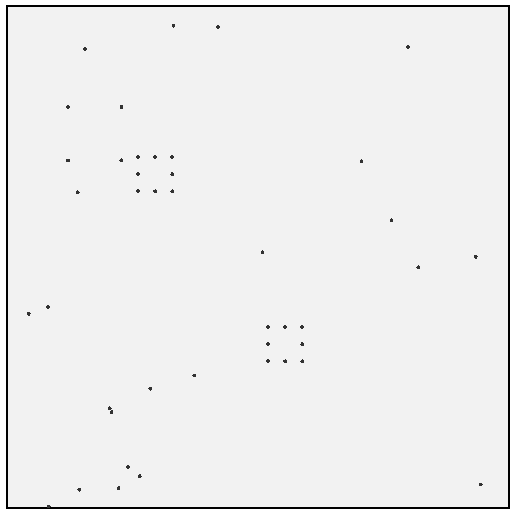
\includegraphics[width=0.44\textwidth]{img/fb60}%
		\qquad\qquad
		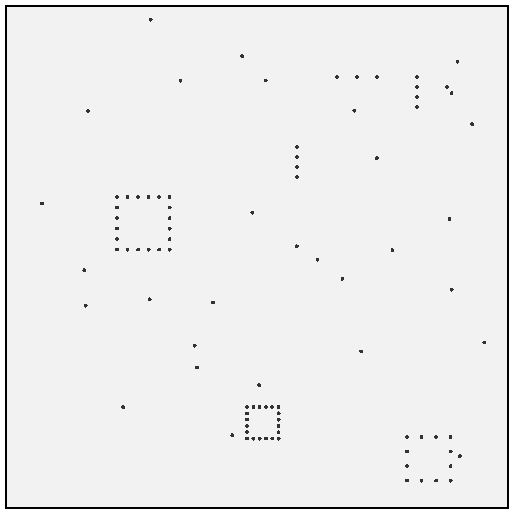
\includegraphics[width=0.44\textwidth]{img/fb100}
		\caption{Random fake PCB with 60 and 100 nodes}
		\label{fig:fakeBoards}
	\end{figure}
\section{First Assignment}

	\subsection{Program}
		In order to resolve the Asymmetric Travelling Salesman Problem with the support of CPLEX API I built three files:
		\begin{itemize}
			\item \verb|main|: the file where all other files are linked and combine in order to solve the problem and use CPLEX API;
			\item \verb|dataReader|: in this file the data is read from a file \verb|.dat| given in input at the start of the program;
			\item \verb|ilpSolver|: this file has the responsibility of initialize the environment of CPLEX API with the \verb|setUp| function, in it all the variables and constraints of the mathematical model are initialize. Instead with the \verb|solve| function the program run the CPLEX method for solving a Mixed Integer Programming Problem.
		\end{itemize}


\section{Second Assignment}

\subsection{Program}
	In order to resolve the Asymmetric Travelling Salesman Problem with meta heuristics, I chose to implement the simple Local Search (LC) and the Tabu Search (TS). This choice was done for two reasons: 
	\begin{itemize}
		\item ;
		\item For test my curiosity about this so simple methods for search a good solution in a ridiculous amount of time.
	\end{itemize}

	From the literature we can see that either LS and mostly TS could be change in every details, starting solution, how to choice the neighbor and so on. For these reason I code the program in a modular way.
	
	For an easier testing I write a class SolverExecutor that groups all Solvers and execute sequentially from the starting solution previously set. With this class is easy to modify the Main.cpp file in order to set the environment of test in a few statements.
	
	The main parts are the Solvers interface implemented by LocalSearchSolver and TabuSearchSolver classes. 
	
	The LocalSearchSolver when creates gives the only option:
	\begin{itemize}
		\item the choice of neighbor: Best improvement and First Improvement.
	\end{itemize}
	
	TabuSearchSolver when creates gives the following options:
	\begin{itemize}
		\item The size of tabu list;
		\item The max number of iteration of the algorithm;
		\item The max seconds of execution;
		\item The choice of neighbor: Best Improvement or First Improvement;
		\item The possibility to enable the Aspiration Criteria, a neighbor in the tabu list is chosen if it has a better value of current best solution.
	\end{itemize}

	\subsubsection{When a move is a Tabu}
		After some test I saw that the 

	
\subsection{Calibration}
	For calibration of the Tabu Search algorithm I look only to the tabu list length parameter. Hence I evaluate the test by the result obtained in \textbf{20 seconds} (CPU time). In fact if we increase the size of tabu list we need more time for check if one Move is a tabu.
	
	The test ran with 8 different random start solution, the table\ref{tab:TS-calibration} show the results.
	
	
	\begin{table}
		\centering
		\begin{tabular} {l l l l}
			\toprule
			method & tenure & Obj.Value (avg) & CPU time \\
			\midrule
			Tabu Search & & & \\
			 			& & & \\
			 			& & & \\
			\midrule
			TS Aspiration Criteria & & & \\
		\end{tabular}
		\caption{\label{tab:TS-calibration}Risultati calibrazione Tabu Search}
	\end{table}
	
	



	
\section{Tests and Results}

\subsection{Results Exact Method}

\subsection{Results Local Search}

\subsection{Results Tabu Search}

\subsection{Comparisons of results}

\subsection{Comparisons of results}

	Obviously the time of Local search is not comparable to the Exact Method and due to the fact that I set the time for Tabu Search is useless to compare the CPU time between the algorithms used.
	
	Check the differences between the results is much more interesting, figures \ref{fig:comparison} and \ref{fig:fb80-comparison}. We can say that:
	\begin{itemize}
		\item Local Search is the fastest methods.
		\item Tabu Search in almost all cases found the optimal solution or a solution near to optimum;
		\item In general the Tabu Search is better than the Local Search but we need to consider that it requires much more time, 30 seconds versus some milliseconds;
		\item Local Search performs worse for instances with a lot of node.
	\end{itemize}

	\vspace{2cm}
	
	\begin{figure}[bh]
		\centering
		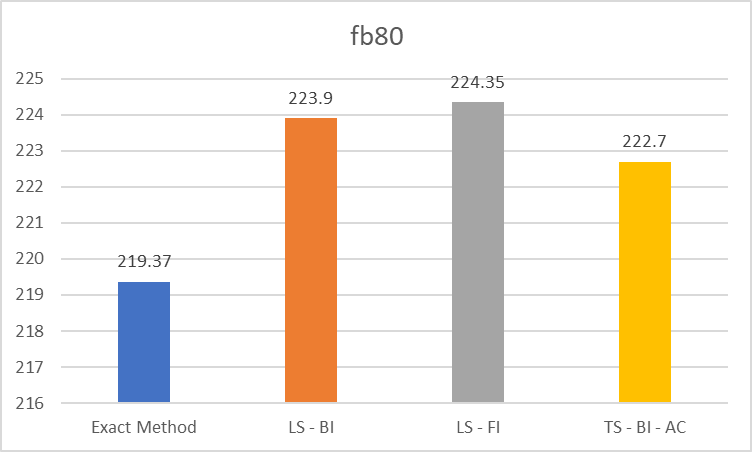
\includegraphics[width=\linewidth]{img/fb80-comparison}
		\caption{Comparison in the fb80 instance. The worse instance for the meta heuristic methods.}
		\label{fig:fb80-comparison}
	\end{figure}
	
	\begin{figure}[h]
		\centering
		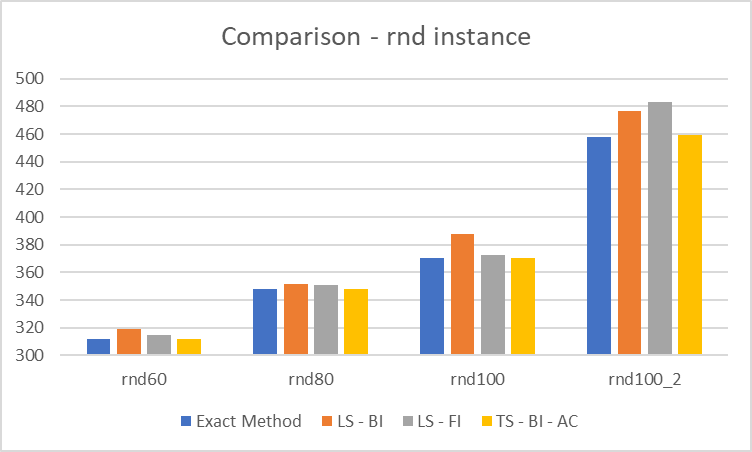
\includegraphics[width=\linewidth]{img/rnd-comparison}

		\vspace{1cm}

		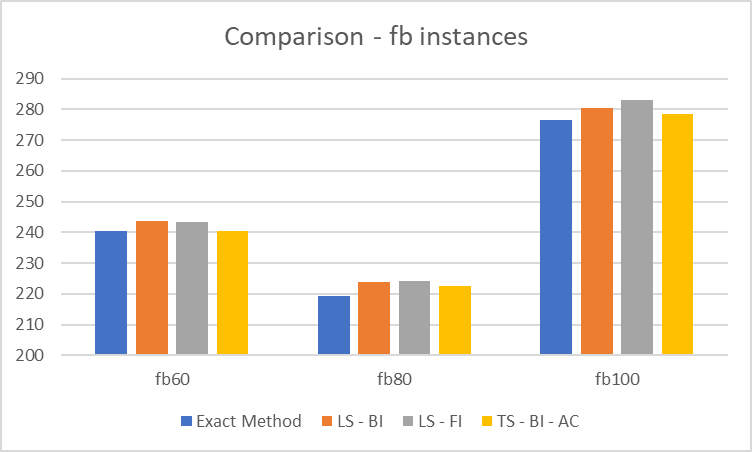
\includegraphics[width=\linewidth]{img/fb-comparison}
		\caption{Comparison of the different methods for rnd and fb instances. \textbf{Note:} in order to mark the difference y-axes doesn't start from 0.}
		\label{fig:comparison}
	\end{figure}

	
	
	
\section{Real Domain tests}
\label{sec:realDomainTests}
	In order to have a better idea of the quality of the methods previously shown I tested them with real instance. These instances are taken from the gerber files avaible from the following online archive:
	\begin{itemize}
		\item \href{https://www.maximintegrated.com/en/design/tools/cad-layout/gerber/}{https://www.maximintegrated.com/en/design/tools/cad-layout/gerber/};
		\item \href{https://www.microchip.com/doclisting/TechDoc.aspx?type=Gerber}{https://www.microchip.com/doclisting/TechDoc.aspx?type=Gerber};
	\end{itemize}

	I explored a dozens of project and select some drill gerber files, from these I made\footnote{This could be done thank to the parser developed by my colleagues Sebastiano Valle and Mirko Bez.} the following \verb|.dat|:
	
	\begin{itemize}
		\item \verb|SC_545|
		\item \verb|MAX_682|
		\item \verb|DS_1120|
	\end{itemize}
	Figure~\ref{fig:SC_545} shows a representation of one of them. The other could be seen from the pdf inside the \verb|RealInstances| folder attached to this report.

	\begin{figure} [h]
		\centering
		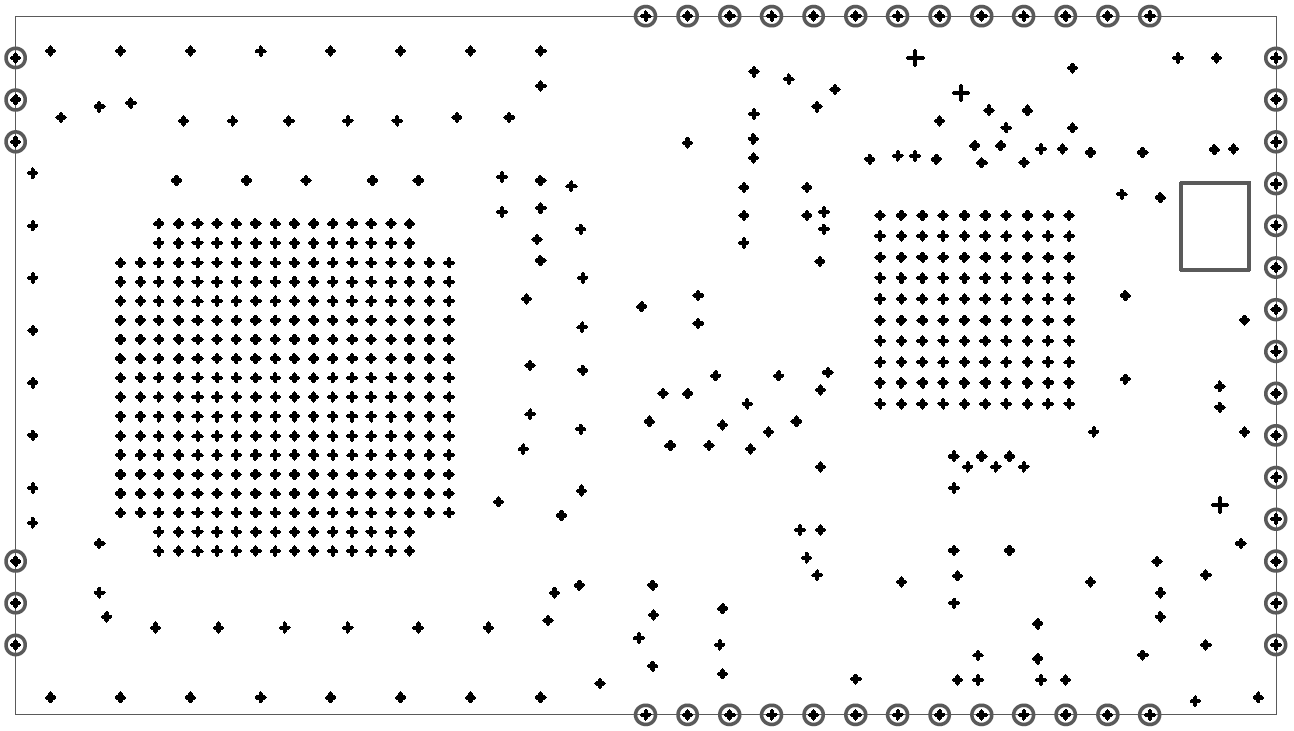
\includegraphics[width=\textwidth]{img/SC_545}
		\caption{The representation of the SC\_545 real instance.}
		\label{fig:SC_545}
	\end{figure}
	
	
	
	\subsection{Results exact method}
		The instances are too huge and the power of computation is too low in order to test the exact method implemented with CPLEX in an amount of time for this project purpose. Neither with a time-out the CPLEX API can give me a intermediate solution in a reasonable amount of time.
		
	\newpage
	
	\subsection{Results Local Search}
		I run the local search with the \textbf{strategy} explained in the previous section \ref{subsec:results-ls}.
		
		
	
	
	\newpage
	
	\subsection{Results Tabu Search}
	
		\subsubsection{Calibration}
			With these new instance the previous calibration is no longer valid. I start from that configuration and I increase the Tabu length.
			
			I made the calibration on \verb|SC_545| instance.
			First I take 8 random initial solution. Then I initialize 4 type of Tabu Search:
			\begin{itemize}
				\item Best Improvement;
				\item Best Improvement with Aspiration Criteria;
				\item First Improvement;
				\item First Improvement with Aspiration Criteria.
			\end{itemize}
			For each type of tabu search I set five different tabu length: 100, 180, 240, 300 and 480. Finally I run each Tabu Search with a maximum time of 30 seconds.  Overall I have $4 \cdot 5 \cdot 8 = 160 $ executions. 
			
			The results are shown in the figure \ref{fig:ri-calibration-sc} and \ref{fig:ri-calibration-sc-avg}.
			
			\begin{figure} [hb]
				\centering
				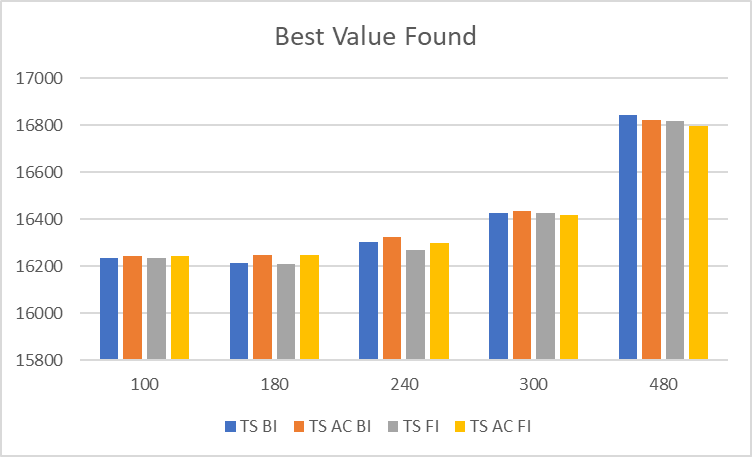
\includegraphics[width=\linewidth]{img/RI-calibration-SC}
				\caption{Calibration Real Instances - best value found.}
				\label{fig:ri-calibration-sc}
			\end{figure}

\newpage	
	
		\begin{figure}[ht]
			\centering
			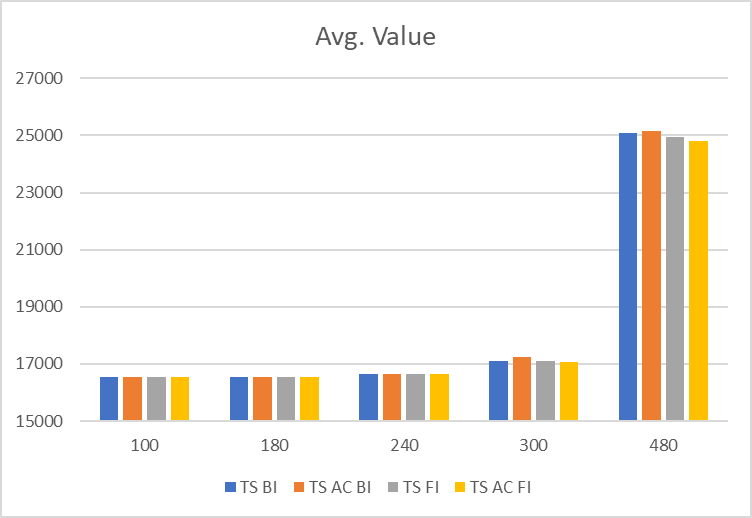
\includegraphics[width=\linewidth]{img/RI-calibration-SC-avg}
			\caption{Calibration Real Instances - Average value}
			\label{fig:ri-calibration-sc-avg}
		\end{figure}
		
			From the charts we can observe that there is some particular differences between the types of Tabu Search. 
			Furthermore we can observe that increasing the tabu length decrease the best value found and also the average of value found. This is suspected, in fact, with tabu length equal to 480, we obtain these because with a tabu list too long the program have a performance bottleneck in the check if a move is a tabu. Hence I start another calibration, only for TS BI AC (choose arbitrarily) with a tabu length equal to 480 and with a maximum time of 300 seconds (5 minutes).
			
			The figure \ref{fig:ri-calibration-tabulengthintime} show with evidence that with more time a larger tabu length is better. If we run a tabu search with tabu length equal to 180 and with a maximum time of 300 seconds we obtain a little improvement but not as the improvement for 480 tabu length case.
			
			\paragraph*{Optimize the code} In order to improve the check if a move is a tabu I substitute the tabu list with two data structures. First I use a \verb|std::list| in order to keep the order of moves inserted into the tabu list. With this data structure I can remove the first element and push back at constant time.
			Second I use a \verb|std::set| for check if a move is a tabu in constant time. I use the concatenation of integer \verb|from| and \verb|to| as key.
			
			\textbf{N.B.} This optimization could brings better result in all the previously test. For limit of time I use the optimization only from now on.
			
			\paragraph*{} With the implementation I execute again some test with TS BI AC with tabu length 180 and 480. The result is that now with 30 seconds I can achieve a better result with tabu length of 480, also the tabu length of 180 have a better solution. In figure ~\ref{fig:ri-calibration-optimize} are shown the comparison between before and after optimization. 
			
			
\newpage		
	
			\begin{figure}
				\centering
				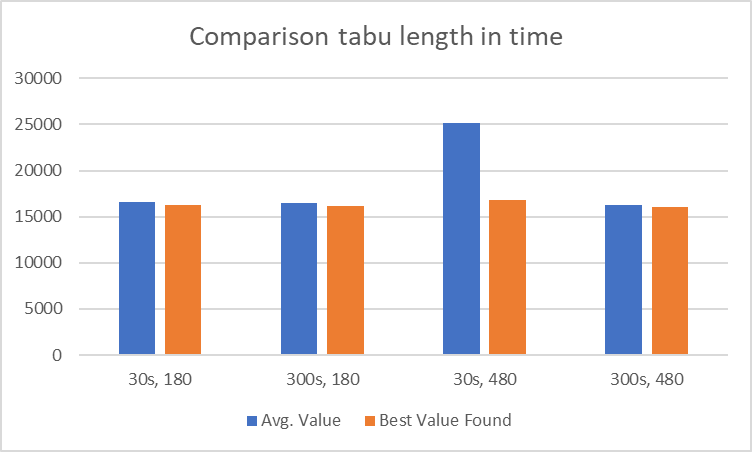
\includegraphics[width=\linewidth]{img/RI-calibration-TabuLengthInTime}
				\caption{Comparison results of TS BI AC with different tabu length and max time.}
				\label{fig:ri-calibration-tabulengthintime}
			\end{figure}
		
			\begin{figure}
				\centering
				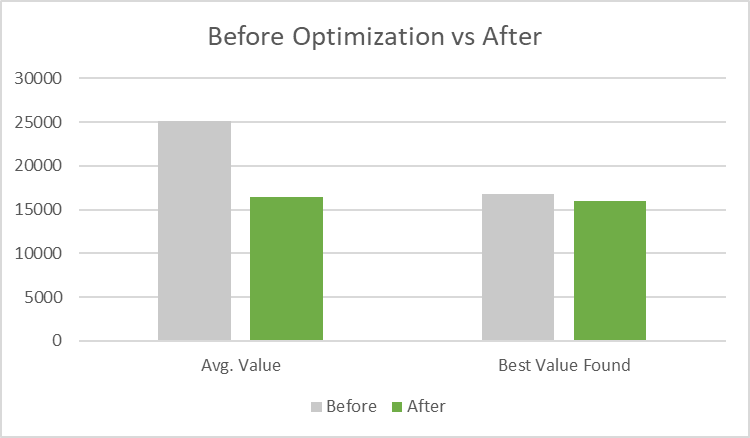
\includegraphics[width=\linewidth]{img/RI-calibration-optimize}
				\caption{Result of TS BI AC in 30 seconds, length of 480, without and with optimization of tabu list.}
				\label{fig:ri-calibration-optimize}
			\end{figure}
		
		
			
			
		
			
			
		
			
		
			
			
			
	
	
	
		
		
	

\subsection{Comparison of results}
	
	From the table~\ref{tab:ri-comparison-results} we can see that for \verb|SC_545| and \verb|MAX_682| the Tabu Search is the best choice but it needs 8 minutes of computation versus only a few seconds of Local Search. In the \verb|DS_1120| instance instead Tabu Search performs poorly, this happens because the 60 seconds for each run it's not a sufficient time to get a local minimum. I think this is due to the fact that with 1120 nodes the evaluation of neighbours needs much more time than with others instances.

	\begin{table}[hb]
		\centering
		\begin{tabular}{llrrrr}
			\toprule
			\textbf{Instance} & \textbf{Solver} & \textbf{Avg Value} & \textbf{Best Value} & \textbf{Avg T (s)} & \textbf{Tot T (s)} \\
			\toprule
			\verb|SC_545|           & TS BI AC        & 16250.2            & 15991               & 60.01                 & 480.06                \\
			& LS BI           & 16809.8            & 16440               & 0.45                  & 3.59                  \\
			& LS FI           & 16504.8            & 16231               & 0.70                  & 5.61                  \\
			\midrule
			\verb|MAX_682|          & TS BI AC        & 5276730.0          & 5115970             & 60.02                 & 480.12                \\
			& LS BI           & 5350680.0          & 5187620             & 0.86       &  6.92           \\
			& LS FI           & 5356200.0          & 5272060             & 1.44                 &   11.56                \\
			\midrule
			\verb|DS_1120|          & TS BI AC        & 35080600.0         & 33428000            & 60.04                 & 480.36                \\
			& LS BI           & 17051200.0         & 16969100            & 4.99                & 39.94                \\
			& LS FI           & 16921800.0         & 16742900            & 8.88                & 71.01    \\
			\bottomrule             
		\end{tabular}
		\caption{Comparison of results between Local Search and Tabu Search with real instances (T = Time).}
		\label{tab:ri-comparison-results}
	\end{table}
\section{Conclusion}

	\paragraph{Use Meta Heuristics}
	Domain context:
		if it's needed a quickly response (think about a user using a CAD/CAM);
		if the cycle of update on the PCB files is fast, it's better to use a Meta Heuristics method.
		If the company don't produce huge amount of a single board.
		
	\paragraph{Use Exact Method}
		Instead if the number of boards produced s huge and the production continue for long period in that case is better to invest time and resources in order to get the optimal solution with an exact method.
\appendix
\section{Instructions for run programs}




\section{How to not optimize the Tabu List}
	In this section I try to understand how different implementations of Tabu list for the Tabu Search method can impact in the quality of the best solution found in a certain amount of time. I also compared the results with the results of the Local Search method.

\subsection{Tabu Search Algorithm}
	I focus my test only on the Tabu Search Best Improvement hence I remove all the others stuff: some switch case and the aspiration criteria.
	The Tabu Search Algorithm is implemented as the Local Search algorithm and it add some operations for managing the tabu list:
	\begin{itemize}
		\item in the choice of a neighbour move it check if that move is into the tabu list;
		\item after the computation of the move it push back the move done and if the tabu list reach the maximum size it pop the front move from the tabu list;
		\item the iteration process is stopped if the time is greater than the maximum time set.
	\end{itemize}
	All the other parts of the algorithm are equal to the Local Search implementation.
	
	
	
	%\begin{itemize}
	%	\item At each iteration if Tabu list size is less of tabu length set the algorithm push back the \verb|TSPMove| into the list;
	%	\item otherwise the algorithm pop the front of the list and
	%\end{itemize}

	\subsection{Implementations variants of Tabu List}
		
		\paragraph{std::List} Initially I implemented the Tabu list mechanism using a standard \verb|List| container. This sequence container allows constant time in the insertion of a single element (\verb|push_back| method) and in the erase of a single element in the front of the list (\verb|pop_front| method)\footnote{from C++11 International Standard §23.3.6.4}.
		The problem with this container is that for checking if a move is a taboo it need $O(n)$ complexity where $n$ is the length of the list.
		
		\paragraph{std::set + std::list} After I detected that with large tabu length the list performs poorly I use a combination of two containers. I use the previously \verb|list| for keeping the order and remove the old move inserted while I use the \verb|set| associative container for get a reduce time of access on my tabu list (now a set). In order to use \verb|set| I encoding a move into a \verb|string|, precisely a concatenation of the two integer \verb|from| and \verb|to|. For example Move of \verb|3| and \verb|7| begin the string \verb|"37"| that I use as key value for the \verb|set|.
		
		\verb|set| container allows insertion  with $N \cdot log (setActualSize + N)$ of complexity, erasing with $log(setActualSize) +  1$ (greater than \verb|List| complexity) but it allows an access with a logarithmic complexity\footnote{C++11 International Standard Table 102 §23.2.4}. 

\subsection{Settings}
\label{subsec:settings}
The following list show the settings for Tabu Search and Local Search:
\begin{itemize}
	\item Best Improvement;
	\item Instance \verb|DS_1120| of 1120 nodes (a restriction due to my time limit);
	\item Maximum computation time 10 seconds;
	\item Four different tabu length values: (the number were chosen keeping in mind the previous report)
	\begin{itemize}
		\item 0;
		\item 20;
		\item 180;
		\item 480.
	\end{itemize}
\end{itemize}

\subsection{Test}
	Since I use the time as stop criteria I decided also to keep in consideration the number of iterations on computation. I consider that more iterations means more probability to find a better value.
	

	
	
	%1
	\paragraph*{}
	In the \textbf{first test} I started the tabu search (settings \ref{subsec:settings}) with \verb|list| and \verb|set+list| with the same initial random solution. The Figure \ref{fig:oneinitrnd} shows that the \verb|set+list| has in all cases a bad performance, instead the \verb|list| goes bad when the list length is large.
	
	This is caused by the fact that the instance \verb|DS_1120| is very large and the convergence on a first local minimum need a lot of iterations (about 1400, result from a Local Search). This could depends on:
	\begin{itemize}
		\item the tabu length, if the length is set to high value the tabu search do diversification;
		\item the time for check if a move is a tabu. For the \verb|set+list| also the time for encoding the move.
	\end{itemize} 
	
	\begin{figure}
		\centering
		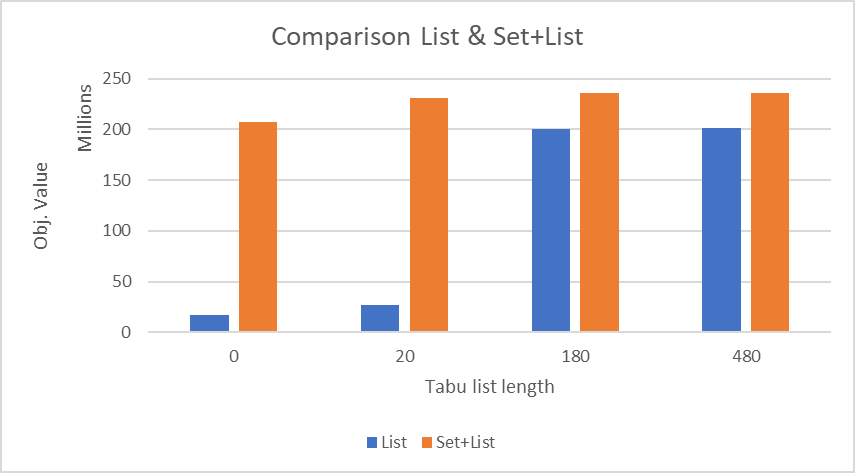
\includegraphics[width=\linewidth]{img/OneInitRnd}
		\caption{Comparison results from list and set+list with search that starts from one random solution.}
		\label{fig:oneinitrnd}
	\end{figure}
	
	
	%2
	\paragraph*{}
	The next test start the tabu search (settings \ref{subsec:settings}) with 8 different initial solution. 10 seconds for each search means a total of 80 seconds for each search execution. In the Table \ref{tab:8initrnd_1} we can see in the column \textbf{Best Value} that \verb|list| found a better solution, unexpectedly the average values for \verb|list| with tabu length 180 and 480 is a lot worse than the average values of \verb|set+list|. The average iterations also indicate that something strange happens with \verb|list|. 
	
	From this strange data a deep inspections on code help me to find a bug in the program. Simply the Tabu Search with \verb|list| executes with the first initial random solution, since the tabu length is big it converges slowly but faster than \verb|set+list| therefore it found a better value than \verb|set+list|. And here the problem comes out: in the next search with another random solution the Tabu list remains the same of the previous search. In this case the converge is even slower cause a lot of move is already tabu and the list is full, that means more time for checking if a move is tabu from the beginning.
	
	In the Table \ref{tab:8initrnd_2} I report the correct data with the bug fixed.
	
	\begin{table}[]
		\centering
		\begin{tabular}{lrrrr}
			\toprule
			\textbf{Data Structure} & \textbf{Length} & \textbf{Avg Value} & \textbf{Best Value} & \textbf{Avg Iterations} \\
			\midrule
			list                    & 0               & 17051200           & 16969100            & 2727                    \\
			& 20              & 26326800           & 25443800            & 825                     \\
			& 180             & 271610000          & 201459000           & 89                      \\
			& 480             & 303803000          & 201459000           & 60                      \\
			\midrule
			set+list                & 0               & 203752000          & 201090000           & 166                     \\
			& 20              & 230667000          & 227666000           & 133                     \\
			& 180             & 241846000          & 234082000           & 120                     \\
			& 480             & 245638000          & 234082000           & 115   \\
			\bottomrule                 
		\end{tabular}
		\caption{Comparison results from list and set+list with search that starts from eight random solution.}
		\label{tab:8initrnd_1}
	\end{table}

	\begin{table}[]
		\centering
		\begin{tabular}{lrrrr}
			\toprule
			\textbf{Solver} & \textbf{Length} & \textbf{Ag Value} & \textbf{Best Value} & \textbf{Avg Iterations} \\
			\toprule
			LS              & -                                   & 17051200                              & 16969100                                & 1388                                        \\
			\midrule
			TS BI list      & 0                                   & 17051200                              & 16969100                                & 2709                                        \\
			& 20                                  & 25677700                              & 24583600                                & 842                                         \\
			& 180                                 & 202994000                             & 200345000                               & 167                                         \\
			& 480                                 & 202713000                             & 200128000                               & 168                                         \\
			\midrule
			TS BI set+list  & 0                                   & 205943000                             & 203128000                               & 163 \\
			& 20                                  & 231721000                             & 228689000                               & 131 \\
			& 180                                 & 236721000                             & 232739000                               & 125  \\
			& 480                                 & 236722000                             & 233591000                               & 125  \\
			\bottomrule
		\end{tabular}
		\caption{Comparison results from LS, TS list and TS set+list with search that starts from eight random solution with the bug fixed.}
		\label{tab:8initrnd_2}
	\end{table}
	

\newpage
		
\subsection{Conclusion}
	Why \verb|set+list| performs so poorly? One fact not take in consideration is the encoding of the \verb|Move| into a string. This operation is very slow with the methods that I used\footnote{Test of different method on different compiler: \\ \href{https://tinodidriksen.com/2010/02/cpp-convert-int-to-string-speed/}{https://tinodidriksen.com/cpp-convert-int-to-string-speed} and also challenges: \\ \href{https://stackoverflow.com/questions/4351371/c-performance-challenge-integer-to-stdstring-conversion}{https://stackoverflow.com/c-performance-challenge-integer-to-stdstring-conversion}.}. 
	Another thing that we need to keep in consideration is that a \verb|set| is a big data structure (a balanced tree) that take about 3 times the memory needed for a simply vector and this means more page faults\footnote{Scott Meyers, Effective STL §3.19.}. This fact maybe justify why the \verb|set+list| performs bad also if tabu length is set to 0, but this fact needs a more deep inspection.
	
	Apart from this stuff about the \verb|set| the main problem on the Tabu Search implemented was the bug where the tabu list was not clear before the start of another search operation. This does not mean that the data collected in the previous report is incorrect, they simply are collected with a special (involuntary) technique where the tabu list was recycled from the previous search at the start of the next search with a different initial random solution. 
	
	In conclusion:
	\begin{itemize}
		\item For small tabu list the standard \verb|list| is more suitable and performs better.
		\item The average of iterations decrease less using a \verb|set+list| than a \verb|list|. In case of the need of a large tabu list, this could be an alternative. In the literature often this is not the case, others container or tricks could performs much better\footnote{hash set is a valid variants of set. Sorted vector often are use as substitute of an associative container.}.
	\end{itemize}
	


\end{document}
